\subsection{Mechanistic Ablation of Muon}
\label{sec:benchmark-muon-ablation}
The benchmark identifies Muon as a strong and mechanistically clean
matrix-structured optimizer. Muon is commonly understood as a momentum-based
matrix optimizer whose key operation is Newton--Schulz (NS)
orthogonalization~\cite{jordan2024muon}. However, this description leaves open
three questions: whether NS is truly indispensable, which auxiliary operations
provide additional gains, and whether the sub-operations can be reordered
freely. We therefore use Muon as a controlled case study for the meta-pipeline
view.

\subsubsection{Single-scene decomposition on C4-350M}
\label{sec}

We first perform a controlled decomposition on C4-LLaMA at the 350M scale,
matching the Stage~1 screening setting. Figure~\ref{fig:muon_ablation_c4_350m}
summarizes the results as absolute validation PPL, where lower is better. The
three blocks correspond to core mechanism recovery, gain design, and
operator-order constraints.

\begin{figure*}[!t]
  \centering
  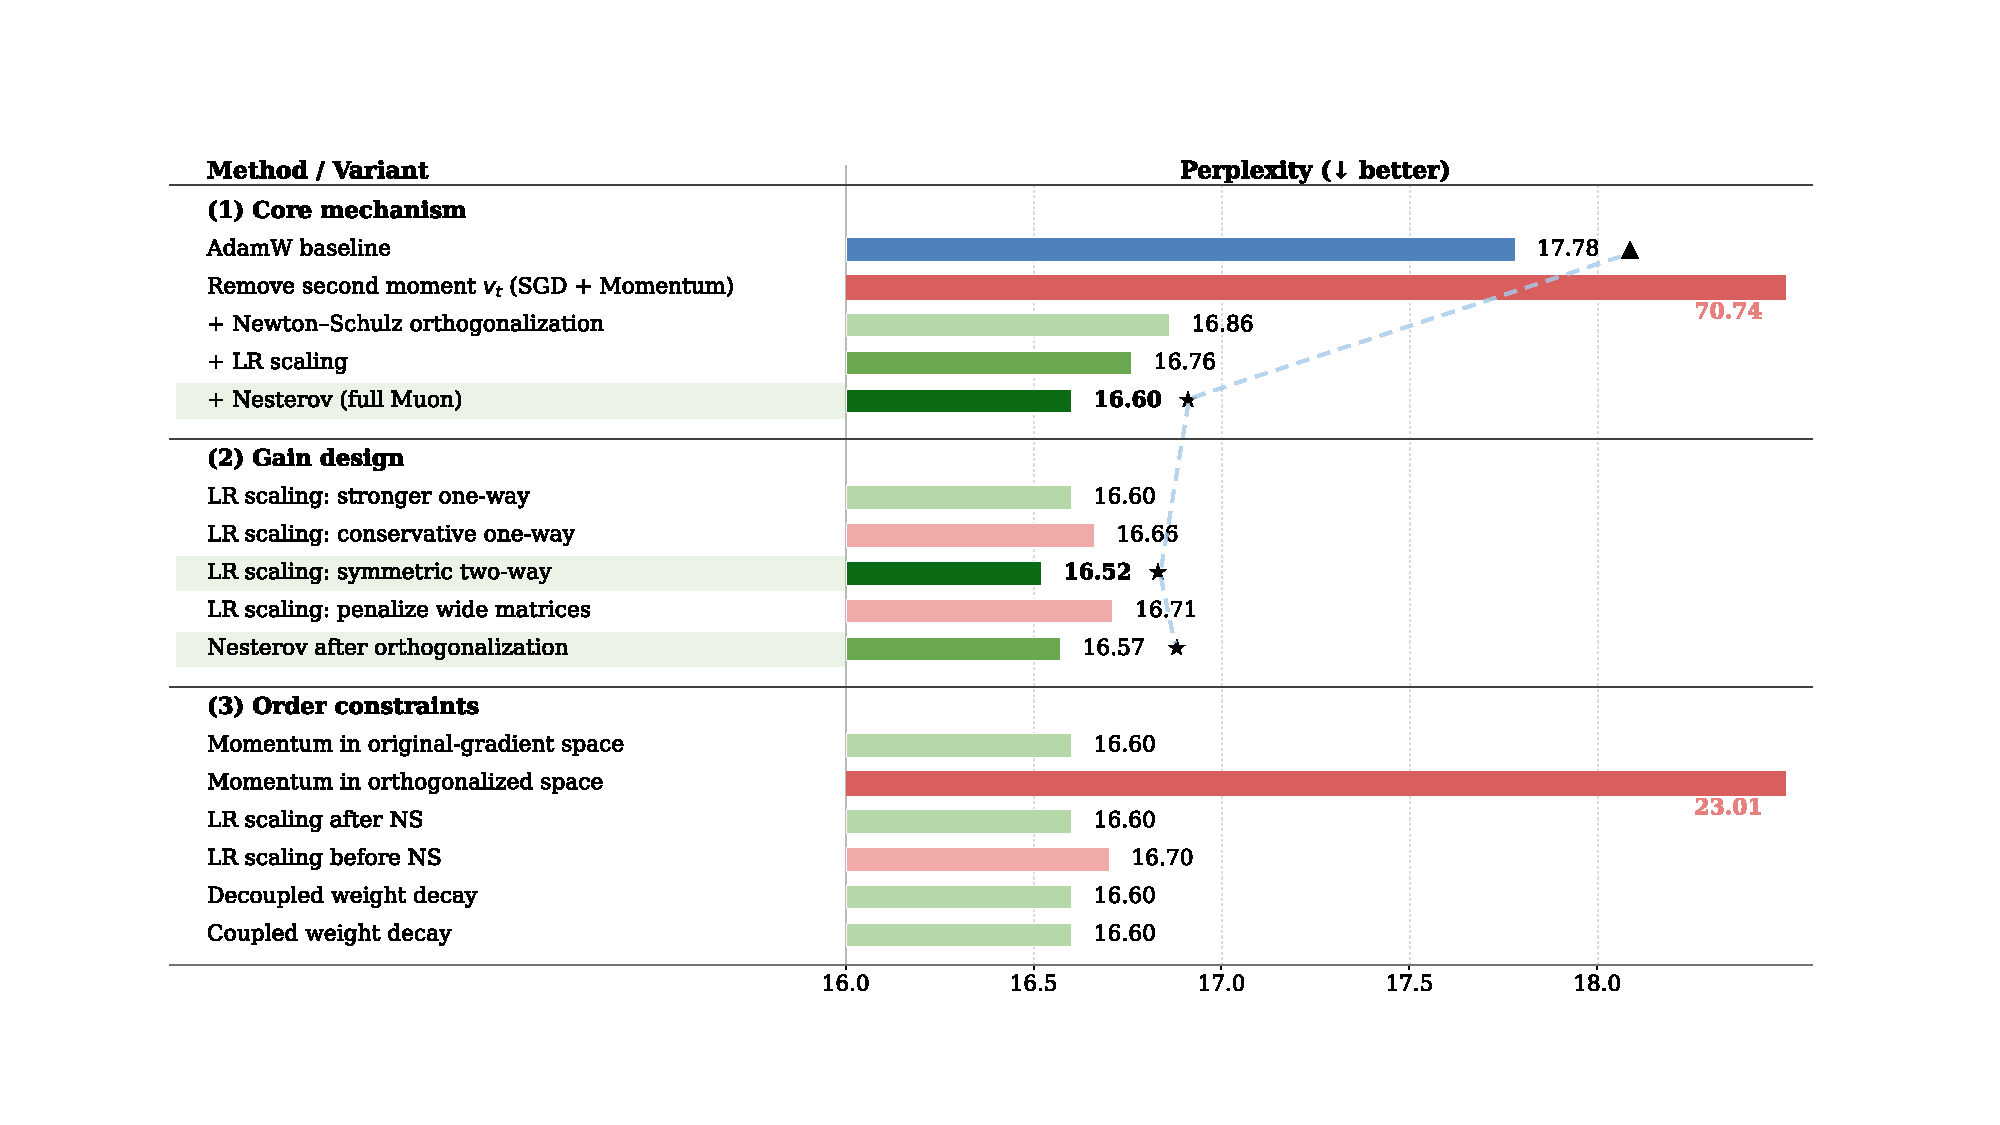
\includegraphics[width=1.0\textwidth]{figures/muon_ablation_c4_350m.pdf}
  \caption{\textbf{Mechanistic ablation of Muon (C4, 350M).} Decomposition into core
operations, gain operations, and operator-order constraints, with bars showing absolute PPL (lower
is better). The 70.74 bar is truncated off-scale.}

  \label{fig:muon_ablation_c4_350m}
\end{figure*}
\paragraph{NS orthogonalization is the core mechanism.}
The first block shows that simply removing AdamW's second moment is
catastrophic, since PPL increases from 17.78 to 70.74. Adding NS orthogonalization
immediately recovers performance to 16.86, already better than AdamW. This
identifies NS as Muon's core replacement for AdamW-style diagonal adaptive
scaling.

\paragraph{Scaling and Nesterov are secondary gains.}
Once NS orthogonalization is present, LR scaling and Nesterov correction
provide smaller but consistent improvements. LR scaling improves PPL from
16.86 to 16.76, and adding Nesterov gives the full Muon result of 16.60.
Thus, these operations refine the orthogonalized direction, but they are not
responsible for the main recovery from the failed no-$v_t$ variant.

\paragraph{The best gains are geometry-aware.}
The second block shows that the form of the gain operation matters. Symmetric
two-way LR scaling gives the best single-scene result, reaching 16.52, whereas
penalizing wide matrices worsens PPL to 16.71. Post-NS Nesterov also improves
over the standard ordering, reaching 16.57. These results suggest that gain
operations should be designed around the geometry of the NS-orthogonalized
direction.

\paragraph{Operator order is constrained.}
The third block shows that Muon's operations are not freely permutable.
Accumulating momentum in the orthogonalized space degrades PPL to 23.01,
whereas accumulating momentum in the original-gradient space keeps PPL at
16.60. Similarly, applying LR scaling before NS worsens PPL to 16.70,
indicating that spectral normalization can absorb or distort the intended
scale correction. Weight-decay ordering is less important in this specific
C4-350M setting, where coupled and decoupled variants are nearly equivalent.

\begin{takeaway}
\noindent\textbf{Single-scene Muon takeaway.}
Muon's main improvement comes from NS orthogonalization, which replaces
AdamW's diagonal second-moment scaling with a matrix-level direction. LR
scaling and Nesterov further refine this direction, but only when placed after
the appropriate upstream operations. The ablation therefore supports the
meta-pipeline view: Muon changes only a few stages, yet the location and order
of those changes are essential.
\end{takeaway}

\subsubsection{Cross-scale and cross-architecture validation}
\label{sec:benchmark-muon-cross-validation}

The single-scene ablation identifies the core and gain operations, but it does
not tell us whether the gain operations transfer. We therefore validate the two
best gains---symmetric two-way LR scaling and post-NS Nesterov---across scale
and architecture. Table~\ref{tab:muon_cross_validation} compares standard
Muon, each gain alone, and their combination on C4-LLaMA at 350M and 1B, as
well as on FineWeb-Edu 32k with Gated DeltaNet at 340M.

\begin{table}[t]
\centering
\vspace{-0.25em}
\caption{\textbf{Cross-scale and Cross-Architecture Validation for Gain Operations in Muon.} Standard Muon, symmetric two-way LR scaling, post-NS Nesterov, and their combination; lower PPL is better. Gains stack on the standard Transformer but not on Gated DeltaNet.}
\label{tab:muon_cross_validation}
\small
\setlength{\tabcolsep}{6pt}
\renewcommand{\arraystretch}{1.14}
\resizebox{0.95\linewidth}{!}{
\begin{tabular}{lccccc}
\toprule
\textbf{Scenario}
& \makecell{\textbf{Standard}\\\textbf{Muon}}
& \makecell{\textbf{Symmetric}\\\textbf{LR Scaling}}
& \makecell{\textbf{Post-NS}\\\textbf{Nesterov}}
& \makecell{\textbf{Both}\\\textbf{combined}}
& \textbf{Best config.} \\
\midrule
\multicolumn{6}{l}{\textit{Standard Transformer: gains are stackable}} \\
C4-LLaMA, 350M
& 16.60
& 16.52
& 16.57
& \bestnum{16.51}
& Both combined \\
C4-LLaMA, 1B
& 13.72
& 13.64
& 13.64
& \bestnum{13.58}
& Both combined \\
\midrule
\multicolumn{6}{l}{\textit{Linear attention: stacking effect disappears}} \\
\rowcolor{warnbg!35}
FineWeb-Edu 32k, GDN-340M
& 24.26
& \bestnum{24.02}
& 24.12
& 24.12
& Symmetric LR Scaling \\
\bottomrule
\end{tabular}}

\end{table}
On standard Transformer models, the two gains are transferable and partially
stackable. At 350M, symmetric LR scaling improves PPL from 16.60 to 16.52,
post-NS Nesterov reaches 16.57, and combining both gives 16.51. At 1B, both
individual gains reach 13.64, and the combined variant further improves to
13.58. This indicates that the two gains act through mostly separable
mechanisms on standard Transformer architectures.

On Gated DeltaNet, the behavior is different. Both gains remain useful
individually, with symmetric LR scaling improving PPL from 24.26 to 24.02, and
post-NS Nesterov reaching 24.12. However, their combination no longer improves
over the best single gain, remaining at 24.12. This suggests that the
orthogonality of optimizer components is architecture-dependent, meaning that operations
that are separable on standard Transformers can interact on linear-attention
parameter topologies.

\begin{takeaway}
\noindent\textbf{Cross-validation takeaway.}
The Muon gains transfer across scale on standard Transformers, but lose
additivity on Gated DeltaNet. Thus, LR scaling and post-NS Nesterov are useful
refinements, but their interaction depends on the target architecture. This
explains Muon's role in the benchmark: it is not a universally best optimizer,
but it is strong, interpretable, and exposes where matrix-structured optimizer
design meets model topology.
\end{takeaway}